In this section we will prove that if $T$ is a square, the only $n$ to 
make $(T,n)$ a good pair is $1$. We can get an idea to consider general 
questions from this special case. To achieve our goal, we need to consider 
what the shape $\iT_{A1} , \iT_{A_2} ... $ would be by lemma 6, and then 
discuss some situations and details.

In the following discussion if we say lines and points without specified, 
we mean the intersection line segments of domains and the endpoints 
of lines. \newline

\begin{thm}
	The lines which intersect the boundary of the square are perpendicular to the boundary.
\end{thm}

We prove this with lemma 5.

\begin{center}
	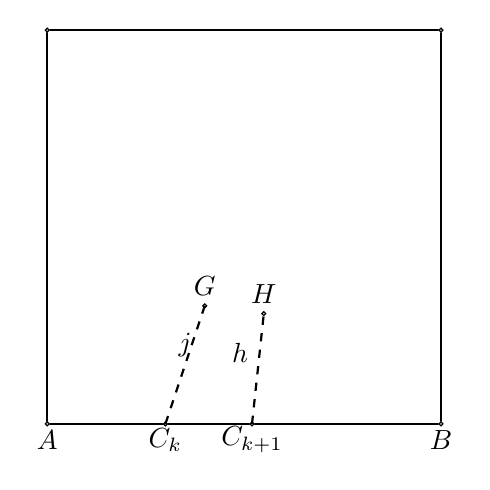
\begin{tikzpicture}[scale=0.5]
	
	\draw[thick][black](0,0)--(10,0)--(10,10)--(0,10)--cycle ;
	
	
	\draw[fill][lightgray](0,-0) circle [radius=0.05];
	\draw(0,-0) circle [radius=0.05];
	\draw[fill][lightgray](10,0) circle [radius=0.05];
	\draw(10,0) circle [radius=0.05];
	\draw[fill][lightgray](10,10) circle [radius=0.05];
	\draw(10,10) circle [radius=0.05];
	\draw[fill][lightgray](0,10) circle [radius=0.05];
	\draw(0,10) circle [radius=0.05];
	\draw[fill][lightgray](3,0) circle [radius=0.05];
	\draw(3,0) circle [radius=0.05];
	\draw[fill][lightgray](5.2,0) circle [radius=0.05];
	\draw(5.2,0) circle [radius=0.05];
	\draw[fill][lightgray](4,3) circle [radius=0.05];
	\draw(4,3) circle [radius=0.05];
	\draw[fill][lightgray](5.5,2.8) circle [radius=0.05];
	\draw(5.5,2.8) circle [radius=0.05];
	
	\node at (0,-0.4) {$A$};
	\node at (3,-0.4) {$C_k$};
	\node at (5.2,-0.4) {$C_{k+1}$};
	\node at (10,-0.4) {$B$};
	\node at (4,3.5) {$G$};
	\node at (5.5,3.3) {$H$};
	
	\draw[dashed,thick][black](3,0)--(4,3);
	\draw[dashed,thick][black](5.2,0)--(5.5,2.8);
	
	\node at (3.5,2) {$j$};
	\node at (4.9,1.8) {$h$};
	\end{tikzpicture}	
\end{center}


\begin{proof}
	We just consider one side $AB$ of the square.
	
	Let $C_1$, $C_2$... $C_n$ be points on $AB$. For a line $i$ which 
	has an end point on $AB$, call the angle between $i$ and $AB$  
	$\angle iC_iB$.
	
	We will show that for two lines $i$ and $h$ which has endpoints 
	$C_k$ and $C_{k+1}$, the $\angle iAB \leq \angle hAB $. Assume 
	that $i$ is the rightest line which has endpoint $C_k$ and $k$ 
	is the leftest line which has endpoint $C_{k+1}$ (or we can 
	compare the rightest line which has endpoint $C_k$ and the 
	leftest line which has endpoint $C_{k+1}$ first). $i$ and $h$ 
	are the sides of the same domain. Because this domain is centrally 
	symmetric and convex, we get that $\angle iC_kC_{k+1}+\angle 
	hC_{k+1}C_{k} \leq \pi$ for any $k$.
	
	We know that the other two adjacent sides of the square are both 
	vertical with $AB$, so the inequality we give is taken equal and 
	complete the proof.
\end{proof}

By the theorem above we note that the domain on the sides must be 
rectangles. If we draw it it can be naturally found out that whole 
graph must look like a table, so there is naturally next theorem.

\begin{center}
	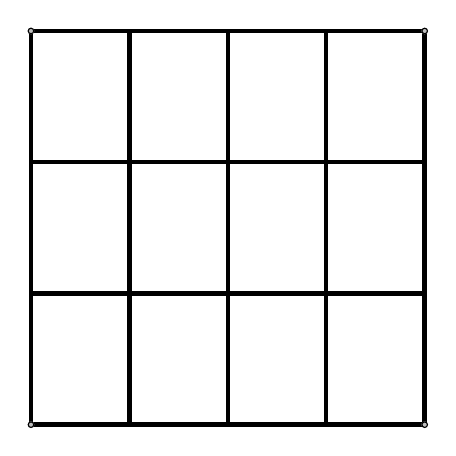
\begin{tikzpicture}[scale=0.5]
	\draw[ultra thick][black](0,0)--(10,0)--(10,10)--(0,10)--cycle ;
	\draw[fill][lightgray](0,-0) circle [radius=0.07];
	\draw(0,-0) circle [radius=0.07];
	\draw[fill][lightgray](10,0) circle [radius=0.07];
	\draw(10,0) circle [radius=0.07];
	\draw[fill][lightgray](10,10) circle [radius=0.07];
	\draw(10,10) circle [radius=0.07];
	\draw[fill][lightgray](0,10) circle [radius=0.07];
	\draw(0,10) circle [radius=0.07];
	
	\draw[ultra thick][black](0,3.33333)--(10,3.33333);
	\draw[ultra thick][black](0,6.66666)--(10,6.66666);
	\draw[ultra thick][black](2.5,0)--(2.5,10);
	\draw[ultra thick][black](5,0)--(5,10);
	\draw[ultra thick][black](7.5,0)--(7.5,10);
	
	\end{tikzpicture}	
\end{center}	

\begin{thm}
	If $A_i$ satisfies the conditions, then the domains are 
	congruent rectangles.
\end{thm}

\begin{proof}
	At first we show that the domains on one side are congruent
	rectangles (Picture 1). For any two adjacent domains $\iT_{A_1}$ 
	and $\iT_{A_2}$, the intersection of them must be perpendicular bisector 
	of the two origin points $A_1$ and $A_2$. Thus $\iT_{A_1}$ and 
	$\iT_{A_2}$ are congruent rectangles since they have the same area. 
	Then we prove that all the domains are congruent rectangles (Picture 2). 
	For a rectangle $\iT_{A_3}$ in corner. The symmetric point of $A_3$
	about the topside $A_4$ is another origin point and we can prove that 
	$\iT_{A_4}$ is also a rectangle by using theorem 3.1 again for the
	topside of all the domains on the downside of the square. Then 
	we can prove that $\iT_{A_4}$ is congruent to $\iT_{A_3}$ and 
	we can show that there are a rows of rectangles on the domain 
	of the first row (Picture 3). We can repeat this operation until 
	prove that all the domains are congruent rectangles.
	
	\begin{center}
		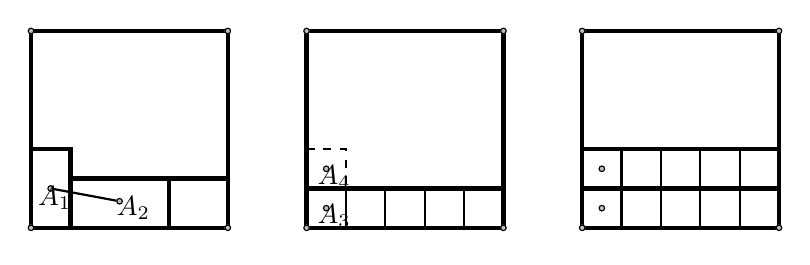
\begin{tikzpicture}[scale=0.5]
		\draw[ultra thick][black](0,0)--(5,0)--(5,5)--(0,5)--cycle ;
		\draw[fill][lightgray](0,-0) circle [radius=0.07];
		\draw(0,-0) circle [radius=0.07];
		\draw[fill][lightgray](5,0) circle [radius=0.07];
		\draw(5,0) circle [radius=0.07];
		\draw[fill][lightgray](5,5) circle [radius=0.07];
		\draw(5,5) circle [radius=0.07];
		\draw[fill][lightgray](0,5) circle [radius=0.07];
		\draw(0,5) circle [radius=0.07];
		
		\draw[ultra thick][black](0,2)--(1,2)--(1,0)--(1,1.25)--(5,1.25)--
		(3.5,1.25)--(3.5,0);
		
		\draw[thick][black](0.5,1)--(2.25,0.675);
		
		\draw[fill][lightgray](0.5,1) circle [radius=0.07];
		\draw(0.5,1) circle [radius=0.07];
		\draw[fill][lightgray](2.25,0.675) circle [radius=0.07];
		\draw(2.25,0.675) circle [radius=0.07];
		\node at (0.6,0.75) {$A_1$};
		\node at (2.6,0.5) {$A_2$};
		
		\draw[ultra thick][black](7,0)--(12,0)--(12,5)--(7,5)--cycle ;
		\draw[fill][lightgray](7,-0) circle [radius=0.07];
		\draw(7,-0) circle [radius=0.07];
		\draw[fill][lightgray](12,0) circle [radius=0.07];
		\draw(12,0) circle [radius=0.07];
		\draw[fill][lightgray](12,5) circle [radius=0.07];
		\draw(12,5) circle [radius=0.07];
		\draw[fill][lightgray](7,5) circle [radius=0.07];
		\draw(7,5) circle [radius=0.07];
		
		\draw[ultra thick][black](7,1)--(12,1);
		
		\draw[thick][black](8,0)--(8,1);
		\draw[thick][black](9,0)--(9,1);
		\draw[thick][black](10,0)--(10,1);
		\draw[thick][black](11,0)--(11,1);
		
		\draw[dashed,thick][black](7,2)--(8,2)--(8,1);
		\draw[fill][lightgray](7.5,0.5) circle [radius=0.07];
		\draw(7.5,0.5) circle [radius=0.07];
		\draw[fill][lightgray](7.5,1.5) circle [radius=0.07];
		\draw(7.5,1.5) circle [radius=0.07];
		\node at (7.7,0.3) {$A_3$};
		\node at (7.7,1.3) {$A_4$};
		
		\draw[ultra thick][black](14,0)--(19,0)--(19,5)--(14,5)--cycle ;
		\draw[fill][lightgray](14,-0) circle [radius=0.07];
		\draw(14,-0) circle [radius=0.07];
		\draw[fill][lightgray](19,0) circle [radius=0.07];
		\draw(19,0) circle [radius=0.07];
		\draw[fill][lightgray](19,5) circle [radius=0.07];
		\draw(19,5) circle [radius=0.07];
		\draw[fill][lightgray](14,5) circle [radius=0.07];
		\draw(14,5) circle [radius=0.07];
		
		\draw[ultra thick][black](14,1)--(19,1);
		\draw[ultra thick][black](14,2)--(19,2);
		
		\draw[thick][black](15,0)--(15,2);
		\draw[thick][black](16,0)--(16,2);
		\draw[thick][black](17,0)--(17,2);
		\draw[thick][black](18,0)--(18,2);
		
		\draw[fill][lightgray](14.5,0.5) circle [radius=0.07];
		\draw(14.5,0.5) circle [radius=0.07];
		\draw[fill][lightgray](14.5,1.5) circle [radius=0.07];
		\draw(14.5,1.5) circle [radius=0.07];
		\end{tikzpicture}	
	\end{center}	
	
\end{proof}

Now it only needs to discuss the situation theorem 3.2 gives.
If $n=1$, it is clear that one can choose $A$ in the middle of the 
square to turn at least half of the square into green. Now we want 
to show that $n=1$ is the only good situation.

If $n>1$, there are only two cases. The one is that the table has 
two or more rows and columns and the other is that it has only one row
or one column.


\begin{center}
	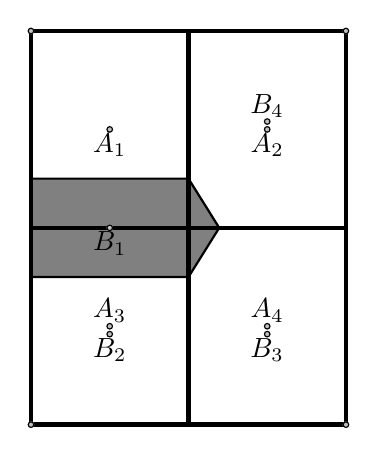
\begin{tikzpicture}[scale=0.5]
	\draw[thick][black][fill=gray](0,6.25)--(4,6.25)--(4.78125,5)
	--(4,3.75)--(0,3.75)--cycle;
	\draw[ultra thick][black](0,0)--(8,0)--(8,10)--(0,10)--cycle ;
	\draw[fill][lightgray](0,-0) circle [radius=0.07];
	\draw(0,-0) circle [radius=0.07];
	\draw[fill][lightgray](8,0) circle [radius=0.07];
	\draw(8,0) circle [radius=0.07];
	\draw[fill][lightgray](8,10) circle [radius=0.07];
	\draw(8,10) circle [radius=0.07];
	\draw[fill][lightgray](0,10) circle [radius=0.07];
	\draw(0,10) circle [radius=0.07];
	
	\draw[ultra thick][black](0,5)--(8,5);
	\draw[ultra thick][black](4,0)--(4,10);
	
	
	
	\draw[fill][lightgray](2,7.5) circle [radius=0.07];
	\draw(2,7.5) circle [radius=0.07];
	\draw[fill][lightgray](6,7.5) circle [radius=0.07];
	\draw(6,7.5) circle [radius=0.07];
	\draw[fill][lightgray](2,2.5) circle [radius=0.07];
	\draw(2,2.5) circle [radius=0.07];
	\draw[fill][lightgray](6,2.5) circle [radius=0.07];
	\draw(6,2.5) circle [radius=0.07];
	
	\node at (2,7.1) {$A_1$};
	\node at (6,7.1) {$A_2$};
	\node at (2,2.9) {$A_3$};
	\node at (6,2.9) {$A_4$};
	
	\draw[fill][lightgray](2,5) circle [radius=0.07];
	\draw(2,5) circle [radius=0.07];
	\draw[fill][lightgray](2,2.3) circle [radius=0.07];
	\draw(2,2.3) circle [radius=0.07];
	\draw[fill][lightgray](6,2.3) circle [radius=0.07];
	\draw(6,2.3) circle [radius=0.07];
	\draw[fill][lightgray](6,7.7) circle [radius=0.07];
	\draw(6,7.7) circle [radius=0.07];
	
	\node at (2,4.6) {$B_1$};
	\node at (2,1.9) {$B_2$};
	\node at (6,1.9) {$B_3$};
	\node at (6,8.1) {$B_4$};
	\end{tikzpicture}	
\end{center}	

For the first case, we consider $4$ rectangles which aligned as
the picture above. Choose the midpoint of $A_1A_3$ as $B_1$ 
and choose $B_2,B_3,B_4$ behind and very close to $A_2,A_3,A_4$
(we can choose them well enough by lemma3). Then $B_1$ changes 
at least $\frac{ab}{2}+\frac{a^3}{16b}$ into green, here $a$ and 
$b$ are the length and width of the rectangle. And $B_2,B_3,B_4$
change almost $\frac{3ab}{2}$ into green. Because $\frac{a^3}{16b}$ is 
a positive number and other points can change $\frac{S_T-ab}{2}
-\epsilon$ into green, then we get contradiction.


\begin{center}
	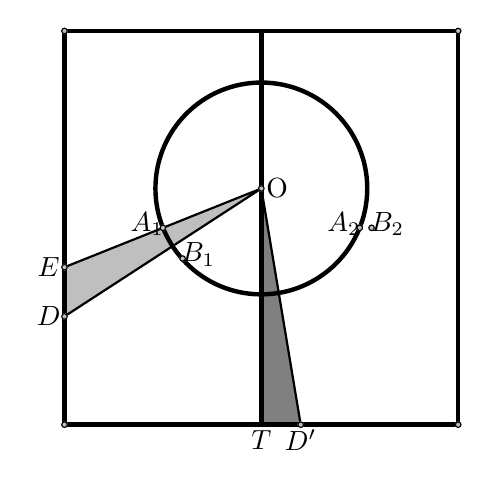
\begin{tikzpicture}[scale=0.5]
	\draw[thick][black][fill=lightgray](5,6)--(0,4)--(0,2.75)--cycle;
	\draw[thick][black][fill=gray](5,6)--(5,0)--(6,0)--cycle;
	
	\draw[ultra thick][black](0,0)--(10,0)--(10,10)--(0,10)--cycle ;
	\draw[fill][lightgray](0,-0) circle [radius=0.07];
	\draw(0,-0) circle [radius=0.07];
	\draw[fill][lightgray](10,0) circle [radius=0.07];
	\draw(10,0) circle [radius=0.07];
	\draw[fill][lightgray](10,10) circle [radius=0.07];
	\draw(10,10) circle [radius=0.07];
	\draw[fill][lightgray](0,10) circle [radius=0.07];
	\draw(0,10) circle [radius=0.07];
	
	
	\draw[ultra thick][black](5,0)--(5,10);
	
	
	\draw[fill][lightgray](5,6) circle [radius=0.07];
	\draw(5,6) circle [radius=0.07];
	\node at (5.4,6){O};
	
	\draw[ultra thick][black](5,6) circle [radius=2.69];
	
	\draw[fill][lightgray](2.5,5) circle [radius=0.07];
	\draw((2.5,5) circle [radius=0.07];
	\node at (2.1,5.1) {$A_1$};
	\draw[fill][lightgray](7.5,5) circle [radius=0.07];
	\draw((7.5,5) circle [radius=0.07];
	\node at (7.1,5.1) {$A_2$};
	
	\draw[fill][lightgray](3,4.22) circle [radius=0.07];
	\draw((3,4.22) circle [radius=0.07];
	\node at (3.4,4.32) {$B_1$};
	\draw[fill][lightgray](7.8,5) circle [radius=0.07];
	\draw((7.8,5) circle [radius=0.07];
	\node at (8.2,5.1) {$B_2$};
	
	\draw[fill][lightgray](0,4) circle [radius=0.07];
	\draw((0,4) circle [radius=0.07];
	\node at (-0.4,4) {$E$};
	\draw[fill][lightgray](0,2.75) circle [radius=0.07];
	\draw((0,2.75) circle [radius=0.07];
	\node at (-0.4,2.75) {$D$};
	
	
	
	
	\node at (5,-0.4) {$T$};
	\draw[fill][lightgray](6,0) circle [radius=0.07];
	\draw((6,0) circle [radius=0.07];
	\node at (6,-0.4) {$D'$};
	
	
	\end{tikzpicture}	
\end{center}	

For the second case, select two adjacent rectangles $\iT_{A_1}, 
\iT_{A_2}$. Because the length of the rectangles $a$ are twice
more then there width $b$, we can choose a point $O$ on the 
perpendicular bisector of $A_1A_2$ such that $2|OA_1|<|OT|$ 
by choosing $|OT|$ an suitable number (for example $\frac{5a}{9}$). 
Here $T$ is an endpoint of the intersection line of two domains. 
Let the intersection of $|OA_1|$ and the left side of $\iT_{A_1}$ be $E$,
rotate $OE$ counterclockwise a small angle $\theta$ which makes 
$|OD|\leq|OT|$. Find a point $D'$ on the bottom side of $\iT_{A_2}$
which makes $\angle TOD'$ be $\theta$. Then $S_{EOD} \leq S_{TOD'}$. 
Choose $B$ as the symmetry point of $A_1$ about $OP$.
Call the lower left corner $A_1$ be $F$. Then we find that $B$ changes 
the area $DOD'F$ into green. The area of $DOD'F$ is $S_{TOD'}-S_{EOD}$, 
more than half area of a rectangle. Choose other points suitably to
change $\frac{S_T-ab}{2}-\epsilon$ and we get the contradiction.\newline

Now we have solved the case that $T$ is a square. It shows a basic 
idea to solve the question, and we will see in the next section 
that this example is more important than we think. The idea of the 
first main theorem comes from here and it is a case needed to be 
discussed in the second main theorem.